% ============================================================
%  Section 3: Self-Attention Mechanism
% ============================================================

\section{Self-Attention Mechanism}
\label{sec:attention}

Self-attention is the computational core of \bert{} and the mechanism that enables
every token to directly interact with every other token, regardless of their positional
distance.  Unlike recurrent architectures that process sequences step-by-step, the
self-attention operation is executed in a \emph{single parallelisable pass}, making it
both expressive and computationally efficient on modern hardware.

\subsection{Conceptual Overview}
\label{subsec:attn_concept}

At an intuitive level, self-attention allows the model to ask, for each token
position: \emph{``Given what I am looking for (query), which other tokens in the
sequence (keys) hold the information (values) I should incorporate into my updated
representation?''}  The answer is a \emph{weighted sum} of value vectors, where
the weights reflect the semantic relevance between queries and keys.

This formulation confers three key properties:

\begin{itemize}
  \item \textbf{Global receptive field.}  A token at position $i$ can directly
        attend to a token at position $j$ with $O(1)$ operations, bypassing the
        $O(n)$ path length required by RNNs.

  \item \textbf{Dynamic, content-based weighting.}  Attention weights are computed
        on-the-fly from the current input representations rather than fixed by
        positional priors.

  \item \textbf{Parallelism.}  All attention weights across all positions can be
        computed simultaneously, enabling efficient GPU/TPU utilisation.
\end{itemize}

\subsection{Mathematical Formulation}
\label{subsec:attn_math}

Given an input matrix $\mathbf{X} \in \R^{n \times d}$, three projection matrices
$\mathbf{W}^Q, \mathbf{W}^K \in \R^{d \times d_k}$ and
$\mathbf{W}^V \in \R^{d \times d_v}$ are used to produce:
\begin{equation}
  \mathbf{Q} = \mathbf{X}\mathbf{W}^Q, \quad
  \mathbf{K} = \mathbf{X}\mathbf{W}^K, \quad
  \mathbf{V} = \mathbf{X}\mathbf{W}^V.
  \label{eq:qkv}
\end{equation}
The \emph{scaled dot-product attention} is then:
\begin{equation}
  \operatorname{Attention}(\mathbf{Q}, \mathbf{K}, \mathbf{V})
  = \softmax\!\left(\frac{\mathbf{Q}\mathbf{K}^\top}{\sqrt{d_k}}\right)\mathbf{V},
  \label{eq:attention}
\end{equation}
where the scaling factor $1/\sqrt{d_k}$ prevents the dot products from growing
large in magnitude, which would push the softmax into regions of extremely small
gradients~\cite{vaswani2017attention}.

\begin{remark}
  The raw score matrix $\mathbf{Q}\mathbf{K}^\top \in \R^{n \times n}$ contains one
  scalar score $e_{ij} = \mathbf{q}_i \cdot \mathbf{k}_j$ for every ordered token
  pair $(i, j)$.  Row-wise softmax converts these into a valid probability
  distribution; the output for position $i$ is thus a convex combination of all
  value vectors, weighted by relevance to position $i$.
\end{remark}

\begin{figure}[H]
  \centering
  \begin{minipage}[b]{0.40\textwidth}
    \centering
    \setlength{\fboxrule}{0.8pt}
    \setlength{\fboxsep}{9pt}
    \fbox{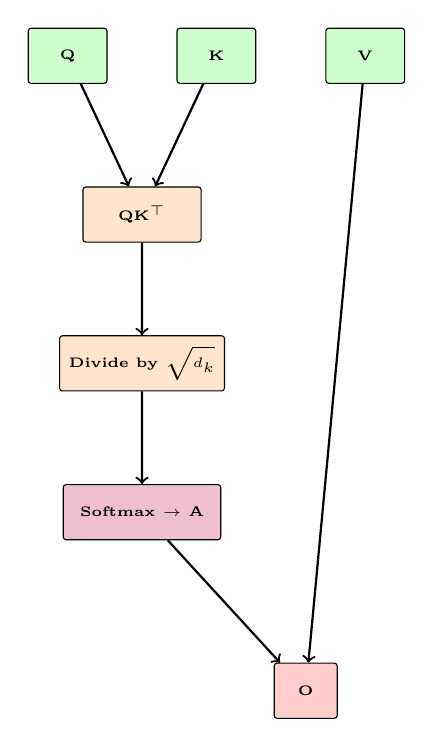
\begin{tikzpicture}[scale=1.26,
        node distance=1.5cm,
        input/.style={draw, fill=green!20, minimum width=1.0cm, minimum height=0.7cm, align=center, font=\tiny\bfseries, rounded corners=1pt},
        op/.style={draw, fill=orange!20, minimum width=1.5cm, minimum height=0.7cm, align=center, font=\tiny\bfseries, rounded corners=1pt},
        attn/.style={draw, fill=purple!25, minimum width=2.0cm, minimum height=0.7cm, align=center, font=\tiny\bfseries, rounded corners=1pt},
        output/.style={draw, fill=red!20, minimum width=0.8cm, minimum height=0.7cm, align=center, font=\tiny\bfseries, rounded corners=1pt}
      ]
      
      % Input layer
      \node[input] (Q) at (0, 4.5) {$\mathbf{Q}$};
      \node[input] (K) at (1.5, 4.5) {$\mathbf{K}$};
      \node[input] (V) at (3.0, 4.5) {$\mathbf{V}$};
      
      % Compute scores
      \node[op] (scores) at (0.75, 2.9) {$\mathbf{Q}\mathbf{K}^\top$};
      \draw[->, line width=0.8pt] (Q) -- (scores);
      \draw[->, line width=0.8pt] (K) -- (scores);
      
      % Scale
      \node[op] (scale) at (0.75, 1.4) {Divide by $\sqrt{d_k}$};
      \draw[->, line width=0.8pt] (scores) -- (scale);
      
      % Softmax → Attention weights
      \node[attn] (attn) at (0.75, -0.1) {Softmax $\to$ $\mathbf{A}$};
      \draw[->, line width=0.8pt] (scale) -- (attn);
      
      % Multiply by V and output
      \node[output] (output) at (2.4, -1.9) {$\mathbf{O}$};
      \draw[->, line width=0.8pt] (attn) -- (output);
      \draw[->, line width=0.8pt] (V) -- (output);
      
    \end{tikzpicture}}
    \subcaption{Scaled Dot-Product Attention}
    \label{fig:sdpa}
  \end{minipage}
  \hfill
  \begin{minipage}[b]{0.58\textwidth}
    \centering
    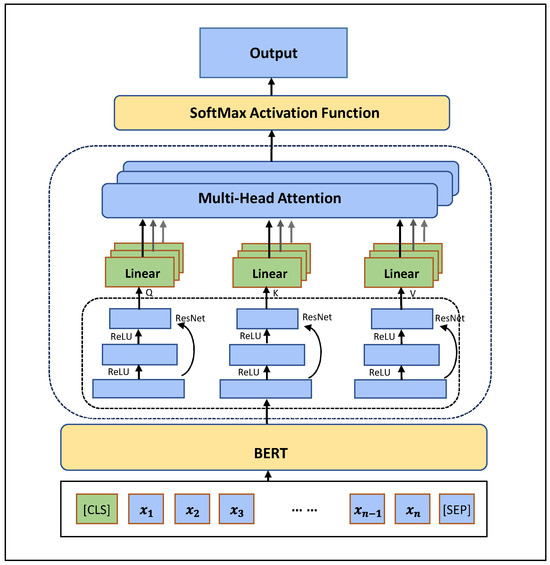
\includegraphics[width=\textwidth]{figures/multiheadattention.jpg}
    \subcaption{Multi-Head Attention}
    \label{fig:mha}
  \end{minipage}
  \caption{Attention mechanisms in BERT. (Left) Scaled dot-product attention computes relevance scores from queries and keys, applies softmax normalization to obtain attention weights $\mathbf{A}$, then aggregates values. (Right) Multi-head attention applies $h$ parallel scaled dot-product functions in projected subspaces.}
  \label{fig:attention_mechanisms}
\end{figure}

\subsection{Interpretation of Query, Key, and Value Roles}
\label{subsec:attn_roles}

\begin{itemize}
  \item \textbf{Queries} encode what a given token is \emph{seeking} from the rest
        of the sequence.
  \item \textbf{Keys} encode what information each token \emph{offers} to other
        positions.
  \item \textbf{Values} carry the actual \emph{content} to be aggregated into the
        output representation.
\end{itemize}

\noindent This abstraction is inspired by retrieval systems in information theory and
provides a powerful inductive bias for relational reasoning over sequences.

\subsection{Multi-Head Attention}
\label{subsec:multihead}

Rather than computing a single attention function, \bert{} employs $A$ parallel
\emph{attention heads}, each operating in a lower-dimensional subspace
$d_k = d_v = d/A$:
\begin{equation}
  \operatorname{head}_a = \operatorname{Attention}(
    \mathbf{Q}\mathbf{W}_a^Q,\;
    \mathbf{K}\mathbf{W}_a^K,\;
    \mathbf{V}\mathbf{W}_a^V
  ), \quad a = 1, \ldots, A.
  \label{eq:head}
\end{equation}

\begin{table}[H]
  \centering
  \caption{Attention head configuration for standard \bert{} models.  Each head
           operates independently in a projected subspace before concatenation.}
  \label{tab:attention_heads}
  \renewcommand{\arraystretch}{1.3}
  \begin{tabular}{lccccc}
    \toprule
    \textbf{Model} & $d$ & $A$ & $d_k$ & $d_v$ & Params/Head \\
    \midrule
    \bert{}-Base  & 768  & 12 & 64  & 64  & $\approx$49K \\
    \bert{}-Large & 1024 & 16 & 64  & 64  & $\approx$65K \\
    \bottomrule
  \end{tabular}
\end{table}
The outputs of all heads are concatenated and projected back to dimension $d$:
\begin{equation}
  \operatorname{MHSA}(\mathbf{Q}, \mathbf{K}, \mathbf{V})
  = \bigl[\operatorname{head}_1 \;\|\; \cdots \;\|\; \operatorname{head}_A\bigr]
    \mathbf{W}^O,
  \label{eq:multihead}
\end{equation}
where $\mathbf{W}^O \in \R^{d \times d}$ is an output projection matrix.  Multiple
heads allow the model to simultaneously attend to information from different
representational subspaces --- e.g., one head may specialise in syntactic
subject–verb relations while another focuses on coreference.

\subsection{Position-Wise Feed-Forward Network}
\label{subsec:ffn}

Following the multi-head attention sub-layer, each encoder layer applies an
identical two-layer feed-forward network independently to each token position:
\begin{equation}
  \operatorname{FFN}(\mathbf{x})
  = \gelu(\mathbf{x}\mathbf{W}_1 + \mathbf{b}_1)\mathbf{W}_2 + \mathbf{b}_2,
  \label{eq:ffn}
\end{equation}
where $\mathbf{W}_1 \in \R^{d \times d_{\mathrm{ff}}}$,
$\mathbf{W}_2 \in \R^{d_{\mathrm{ff}} \times d}$, and the inner dimension is
$d_{\mathrm{ff}} = 4d$ (e.g., 3072 for \bert{}-Base).  The $\gelu$ activation
function~\cite{hendrycks2016gelu} is a smooth approximation to ReLU that has been
found to perform better empirically in deep Transformers.
